% begin module infinite-limit-at-infinity-ex11
\begin{frame}
\begin{example}%[Example 11, p. 237]
Find the limits as $x\to \infty$ and $x\to -\infty$ of $y = (x-2)^4(x+1)^3(x-1)$.
%\begin{columns}[c]
%\column{.5\textwidth}
\begin{center}
\ \only<handout:0| -8>{%
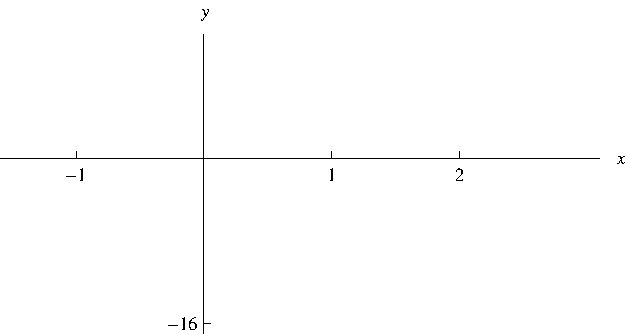
\includegraphics[width=7cm]{curve-sketching/pictures/04-04-ex11a.pdf}%
}%
\only<handout:0| 9-15>{%
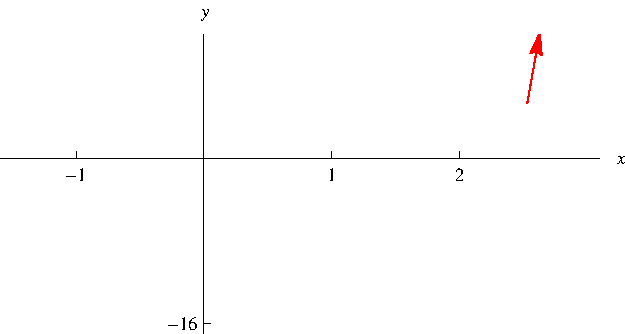
\includegraphics[width=7cm]{curve-sketching/pictures/04-04-ex11b.pdf}%
}%
\only<handout:0| 16>{%
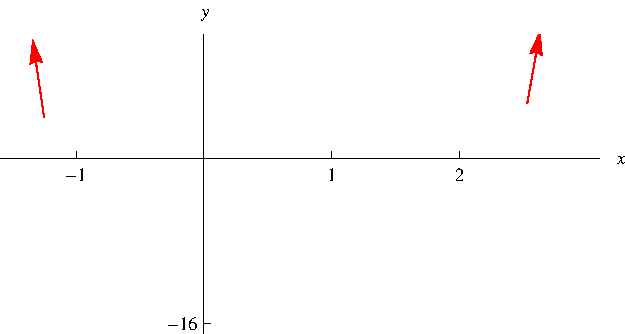
\includegraphics[width=7cm]{curve-sketching/pictures/04-04-ex11c.pdf}%
}%
\only<17->{%
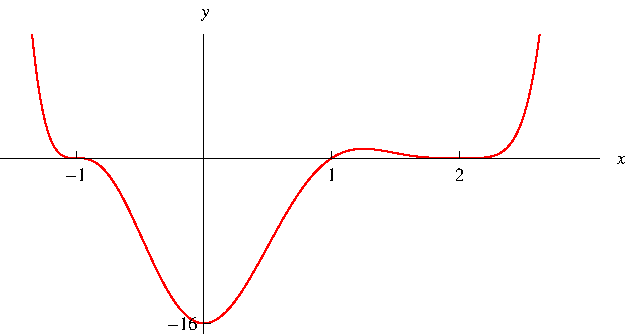
\includegraphics[width=7cm]{curve-sketching/pictures/04-04-ex11d.pdf}%
}%
\end{center}
\uncover<2->{%
\abovedisplayskip=0pt
\belowdisplayskip=0pt
\[
\begin{array}{c@{}c@{}c@{}ccr}
\displaystyle \lim_{x\to \infty}&%
\alert<handout:0| 3-4>{(x-2)^4}&%
\alert<handout:0| 5-6>{(x+1)^3}&%
\alert<handout:0| 7-8>{(x-1)}&%
 = &%
\uncover<9->{\alert<handout:0| 9>{\infty}}%
\\%
&%
\uncover<4->{\alert<handout:0| 4,9>{+}}&%
\uncover<6->{\alert<handout:0| 6,9>{+}}&%
\uncover<8->{\alert<handout:0| 8,9>{+}}&%
&\\%
&&&&&\\%
\displaystyle \lim_{x\to -\infty}&%
\alert<handout:0| 10-11>{(x-2)^4}&%
\alert<handout:0| 12-13>{(x+1)^3}&%
\alert<handout:0| 14-15>{(x-1)}&%
 = &%
\uncover<16->{\alert<handout:0| 16>{\infty}}%
\\%
&%
\uncover<11->{\alert<handout:0| 11,16>{+}}&%
\uncover<13->{\alert<handout:0| 13,16>{-}}&%
\uncover<15->{\alert<handout:0| 15,16>{-}}&%
&%
\end{array}
\]
}%
\vspace{-.1in}
%\end{columns}
\end{example}
\end{frame}
% end module infinite-limit-at-infinity-ex11
